\documentclass{beamer}

\usetheme{metropolis}

\usepackage[utf8]{inputenc}
\usepackage{graphicx}
\usepackage{listings}
\usepackage{xcolor}

\title{Introduction to eBPF}
\author{Théophile Dubuc}
\date{\today}

% Code style
\lstset{
    basicstyle=\ttfamily\footnotesize,
    keywordstyle=\color{blue},
    commentstyle=\color{gray},
    stringstyle=\color{green!50!black},
    numbers=left,
    numberstyle=\tiny\color{gray},
    frame=single,
    breaklines=true,
    postbreak=\mbox{\textcolor{red}{$\hookrightarrow$}\space},
    showspaces=false,
    showtabs=false,
    tabsize=4
}

\begin{document}

\frame{\titlepage}

\section{Introduction: What is eBPF?}
\begin{frame}{What is eBPF?}
    \centering
    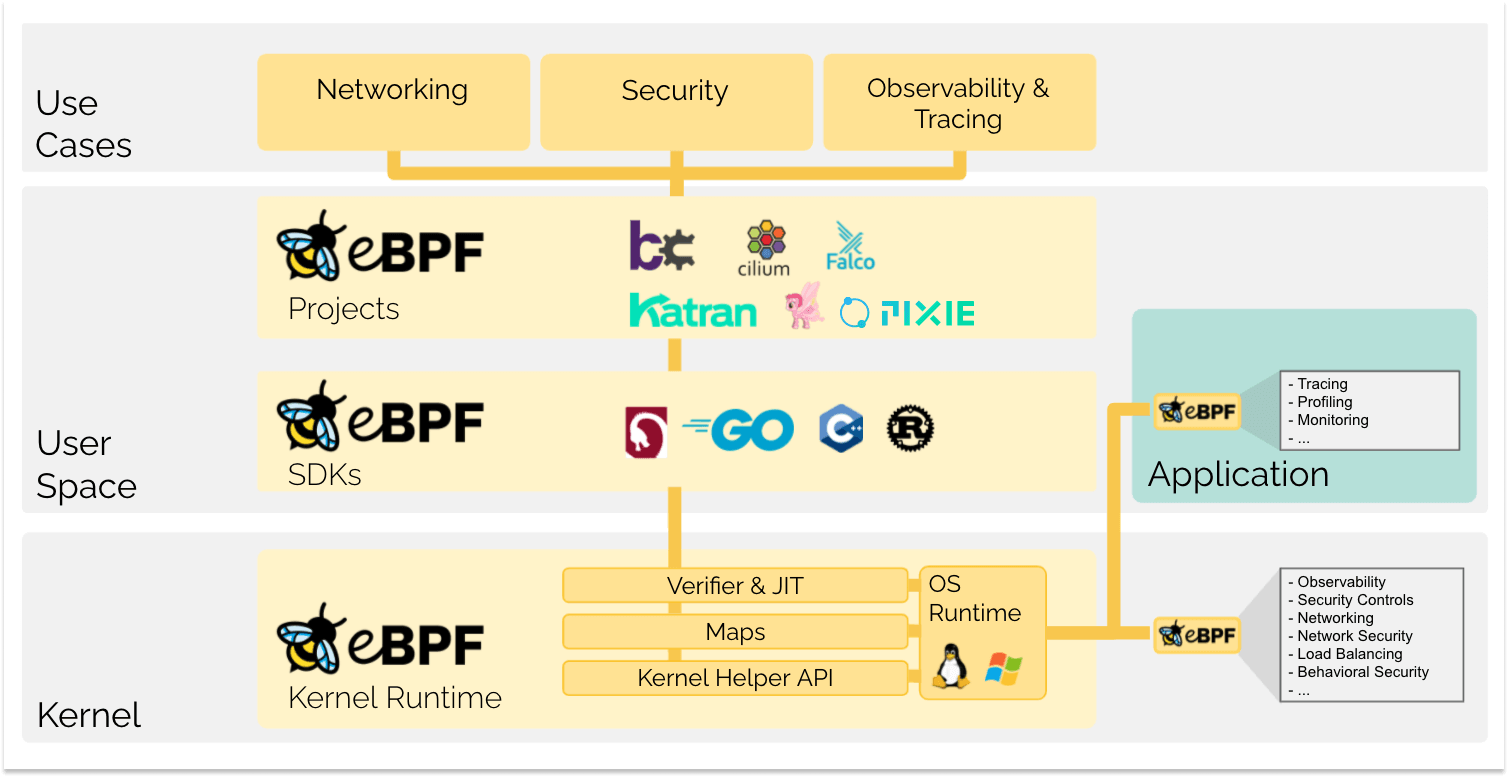
\includegraphics[width=0.8\linewidth]{figures/ebpf-overview.png}
    \begin{itemize}
        \item 1990's: Berkeley Packet Filter (BPF) to filter network packets in
            Unix systems
        \item 2014: extended BPF (eBPF) for the whole kernel
        \item Now, BPF = eBPF and cBPF = old BPF.
        \item Run sandboxed programs in response to kernel events.
        \item Uses cases in observability, security, kernel programming.
    \end{itemize}
\end{frame}

\begin{frame}{How eBPF Works}
    \centering
    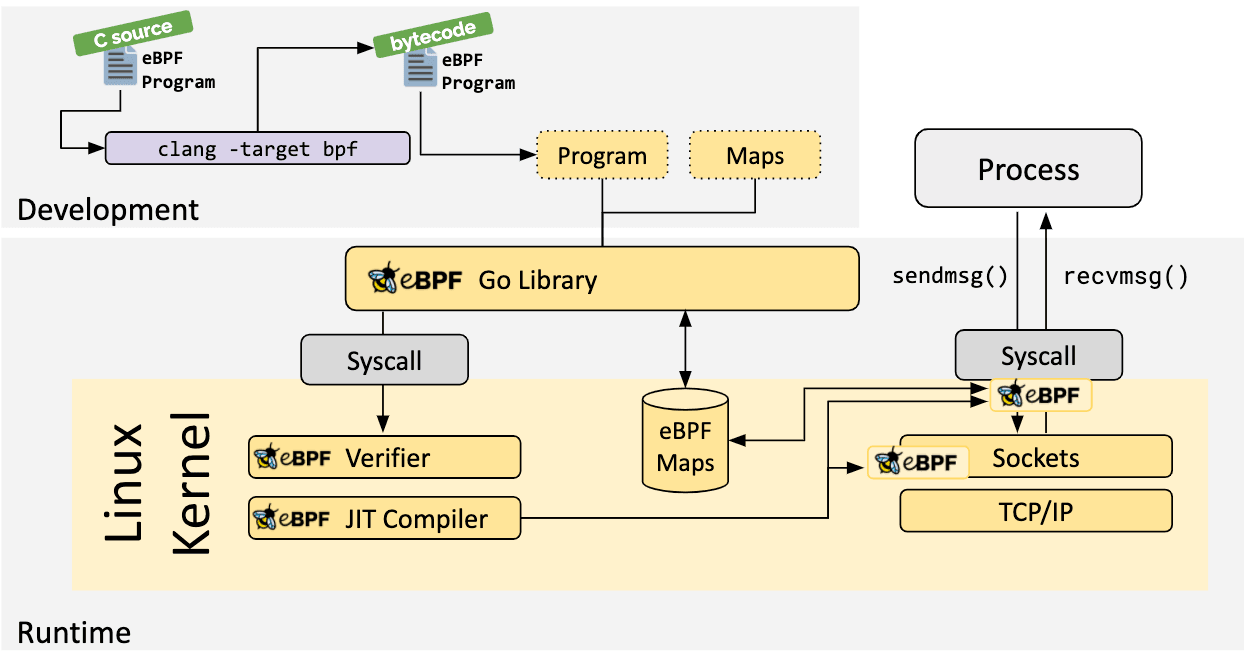
\includegraphics[width=0.8\linewidth]{figures/ebpf-loader.png}
    \begin{itemize}
        \item Load and attach eBPF programs from user space (bpftool, libbpf,
            BCC, etc.).
        \item eBPF program interacts with kernel resources.
        \item Optionally returned to user space via BPF maps, like ring buffers.
    \end{itemize}
\end{frame}

\section{The BPF programming language}
\begin{frame}{The BPF programming language: C with constraints}
    BPF security relies on constraints while programming:
    \begin{itemize}
        \item No standard C libraries, use BPF helpers instead
        \item Limited number of instructions
        \item No "regular" loops
        \item No dynamic memory
        \item Strict pointer checking
        \item No floating point operations
        \item \dots
    \end{itemize}
\end{frame}

\section{Types of eBPF Programs}
\begin{frame}{Tracepoints: Built-In Instrumentation}
    \begin{itemize}
        \item Predefined kernel events.
        \item Lower overhead than kprobes.
        \item Example: monitoring time spent in a syscall.
    \end{itemize}
\end{frame}

\begin{frame}{kprobes: Attaching to Kernel Functions}
    \begin{itemize}
        \item Dynamically attach to almost any kernel function.
        \item Used for:
        \begin{itemize}
            \item Measuring function execution times.
            \item Tracking kernel resource usage.
        \end{itemize}
        \item Example: Hooking \texttt{vfs\_read}.
    \end{itemize}
\end{frame}

\begin{frame}{Attaching to network interfaces}
    Use eBPF like cBPF and perform packet processing by attaching programs to:
    \begin{itemize}
        \item XDP (express data path): very fast, early in the stack
        \item tc (traffic control): more flexible
    \end{itemize}
    With them you perform many operations on ingress and egress packets:
    \begin{itemize}
        \item Read them
        \item Re-write them
        \item Redirect them
        \item Drop them
    \end{itemize}

    And you can offload your programs to compatible NICs!
\end{frame}

\section{Communication Mechanisms}
\begin{frame}{Using \texttt{bpf\_printk}}
    \begin{itemize}
        \item Debugging tool for eBPF programs.
        \item Prints messages to the kernel log (\texttt{dmesg}).
        \item Lightweight but not suitable for production.
    \end{itemize}
\end{frame}

\begin{frame}{Maps: Sharing Data Between Kernel and User Space}
    \begin{itemize}
        \item Key-value storage accessible by both eBPF and user-space programs.
        \item Types:
        \begin{itemize}
            \item Hash maps
            \item Arrays
            \item Per-CPU maps
        \end{itemize}
        \item Example: Counting system calls by process ID.
    \end{itemize}
\end{frame}

\begin{frame}{Ring Buffers: Streaming Data}
    \begin{itemize}
        \item Efficient mechanism for sending structured data to user space.
        \item Commonly used for profiling and tracing applications.
        \item Example: Streaming syscall durations.
    \end{itemize}
\end{frame}

\section*{Conclusion}
\begin{frame}{Summary}
    \begin{itemize}
        \item eBPF provides powerful, low-overhead tools for kernel performance
            evaluation, kernel programming, and packet processing.
        \item Key types of programs:
        \begin{itemize}
            \item kprobes
            \item Tracepoints
            \item Network filters
        \end{itemize}
        \item Communication mechanisms include:
        \begin{itemize}
            \item \texttt{bpf\_printk}
            \item Maps
            \item Ring buffers
        \end{itemize}
    \end{itemize}
    \centering
    \textbf{Lets try it! (Questions before?)}
\end{frame}

\end{document}

